\documentclass{article}

\usepackage[utf8]{inputenc}
\usepackage[top=1in, bottom=1in, left=0.5in, right=0.5in]{geometry}
\usepackage[T1]{fontenc}
\usepackage[frenchb]{babel}
\usepackage{array}
\usepackage{fancyhdr}
\usepackage{amssymb}
\usepackage[final]{pdfpages}
\usepackage{array}

\renewcommand{\baselinestretch}{0.9} 
\setlength\parindent{0pt}

\pagestyle{fancy}
\lhead{Rapport TP3}
\rhead{Minesweeper}

% pour éviter d'avoir à faire des \noindent partout!

\title{%
\Large{Université du Québec à Montréal}\\
\vspace{2.5cm}
\Huge{Minesweeper}\\
\vspace{3cm}
\Large{Travail présenté à \\M. Eric Beaudry} \\
\vspace{2cm}
\Large{Dans le cadre du cours \\INF4230-10 – Intelligence Artificielle}
\author{Martin Bouchard, BOUM15078700\\Frédéric Vachon, VACF30098405\\Louis-Bertrand Varin,
VARL23089000\\Geneviève Lalonde, LALG08568204\\Nilovna Bascunan-Vasquez, BASN22518900}
\date{\vspace{2cm} 15 décembre 2014}
\vfill
}

\begin{document}
\maketitle

\thispagestyle{empty}
\clearpage

\openup .5em

\section{Introduction}
Dans le cadre du troisième TP en Intelligence Artificielle, nous proposons de créer 
un joueur artificiel pour le jeu de démineur (Minesweeper). Afin d’augmenter la complexité 
du projet, nous avons décidé d’implémenter différents algorithmes pour résoudre la 
grille de démineur. L’utilisateur sera en mesure de choisir l’algorithme qu’il désire observer. 

\section{Description du jeu et problématique}
Le jeu démineur appartient à la catégorie des problèmes NP-complets puisqu’il n’est 
pas toujours possible de trouver une solution en temps polynomial. Il n’y a pas de 
méthode connue qui garantisse une meilleure solution que la simple recherche par force 
brute \footnote{Richard Kaynes, Département des Mathématiques, \\ Université de Bimingham http://web.mat.bham.ac.uk/R.W.Kaye/minesw/ordmsw.htm}. 
Ainsi, aucun de nos joueurs artificiels n'est en mesure de garantir une victoire à chaque essaie.
Il s’agit ainsi d’un problème combinatoire souvent intraitable
\footnote{Richard Kaynes, \\ Département des Mathématiques http://web.mat.bham.ac.uk/R.W.Kaye/minesw/minesw.pdf} .

\begin{figure}[h!]
  \caption {Exemple d'une situation non triviale. Les cases bleues sont non découvertes, les chiffres sur les cases découvertes
  représentent le nombre de cases minées adjacentes.}
  \centering
  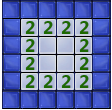
\includegraphics[scale=.5]{./demineur_1.png}
\end{figure}

Dans la figure 1, il faut donc trouver quelles cases parmi les cases non découvertes contiennent des mines. Ici, il y a 
20 cases inconnues et 12 cases qui touchent chacune à 2 mines. En résolvant cette grille, 
nous savons qu’elle contient 8 mines. Dans une approche naïve, où le joueur artificiel 
tenterait toutes les combinaisons possibles à la recherche de la meilleure 
(celle brisant le moins de contraintes) pour une grille non découverte de 6 x 6 
comme celle ci-haut (donc 36 cases), le nombre de combinaisons possibles de 8 mines serait de l’ordre de:
36!/(8!(36-8)!) = 30 260 340. 
Il faut noter que ce chiffre, bien qu’énorme, correspond au nombre de combinaisons d’une grille 
plus petite que le minimum permis dans la version Windows du jeu. \\

La résolution d’une grille de démineur peut être décomposée à la simple question de savoir quelles 
cases sont certaines (d’être minées ou non), et lesquelles sont incertaines. Un bon joueur 
artificiel de démineur ne jouera jamais une case incertaine si des cases certaines 
n’ont pas été jouées. \\

Il s’agit d’un jeu statique à agent unique partiellement observable, dans un environnement 
discret (puisqu’une grille bien délimitée est utilisée). Il s’agit aussi d’un jeu 
déterministe dans la mesure où l’action effectuée par le joueur détermine entièrement 
l’état suivant de la grille. Ce jeu est séquentiel, puisque chaque coup permet de 
découvrir une partie de la grille et restreint potentiellement le domaine des variables du prochain coup.

\section{Heuristiques et pertinence des algorithmes choisis}

Cette section vise à décrire les algorithmes et heuristiques utilisés par nos joueurs artificiels pour
la résolution du jeu de démineur.

\subsection{Heuristiques}

\subsubsection{Délimitation des frontières}
notre joueur artificiel utilise les frontières pour définir 
le domaine des cases candidates pour le prochain coup. Une frontière est 
composée de toutes les cases entourant un indice, et a l’apparence d’un îlot.
                \begin{figure}[h!]
			\caption {délimitation des frontières dans le jeu de démineur.}
                \centering
                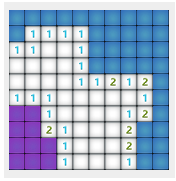
\includegraphics[scale=.5]{./demineur_2.png}
                \end{figure}

\subsubsection{Premier clic}
La première case cliquée par le joueur artificiel sera 
toujours vide (non minée et sans indice), puisqu’il n’y a aucune façon 
d’inférer quelles cases sont minées quand il n’y en a pas une seule de 
découverte. Notre programme construit la grille par la suite, autour de la case jouée.

\subsection{algorithmes}
\subsubsection{Constraint Satisfaction Problem}
Le CSP (Constraint Satisfaction Problem) a servi comme base à tous 
les autres algorithmes, afin d’accélérer la prise de décision en générant 
toutes les dispositions de mines possibles (ce qui permet d’identifier les coups sûrs). 
Les cases du jeu démineur peuvent être représentées comme des variables pouvant adopter 
plusieurs valeurs : minée, sans mine, vide, non-découverte. Puisqu’elles sont gérées 
par des contraintes (e.g deux cases touchant à une case ayant le chiffre 1 ne peuvent 
pas être toutes les deux minées), CSP était tout indiqué pour être utilisé en amont aux autres algorithmes.
Concrètement, la résolution du CSP utilise l'algorithme de Backtracking, avec forward checking afin d’accélérer la génération 
des solutions possibles.

\subsubsection{Choix aléatoire}
La technique primitive du choix aléatoire (utilisée par le joueur artificiel) a été implémentée 
en tout premier pour faciliter les tests et le travail sur l’interface. 
Il s’agit simplement de choisir la prochaine case à jouer parfaitement au hasard. 
Elle est disponible dans les choix d’algorithmes, et est utile pour des fins de comparaison/références.

\subsubsection{Safe or Random AI}
Cet algorithme effectue un simple choix 
aléatoire sur la prochaine case à jouer, quand aucun coup sûr n’est disponible 
(quand notre CSP n’a trouvé aucune case dont le domaine était unique).

\subsubsection{Raisonnement probabiliste simple}
Un algorithme de raisonnement probabiliste (ProbabilisticAI) est aussi disponible. 
Il détermine simplement la probabilité qu’une case soit minée, et utilise une 
PriorityQueue pour stocker les coups à jouer selon leur chance d’être une 
case vide, dans les limites des frontières établies. Lorsque toutes 
les cases candidates ont les mêmes probabilités, il choisit au hasard la prochaine case dans sa Priority Queue.

\subsubsection{Raisonnement probabiliste extérieur}
Ce type de raisonnement probabiliste, utilisé dans Adventurer AI, tient compte des chances à priori qu’une case 
à l'extérieur des frontières découvertes soit une mine. Si cette probabilité est plus intéressante que celles présentes
sur les frontières, un coup à l'extérieur des frontières est joué. Cette technique peut s'avérer très utile en fin de partie.
Par exemple, le coup suivant dévoilant un 4 nous indique qu’il y a 4 mines parmi 
les 8 cases autour de nous (voir image suivante), ce qui signifie que nous avons une chance sur deux de 
tomber sur une mine. Dans une grille où il resterait par exemple 4 mines à découvrir 
sur 60 cases inconnues (donc 15\% des cases restantes étant minées), une case au 
hasard en territoire inconnu aurait environ une chance sur 6 d’être minée, et 
l’aventurier choisirait donc une case au hasard hors de la frontière. 
\begin{figure}[h!]
\caption {Exemple d'une frontière très dangeureuse.}
\centering
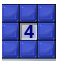
\includegraphics[scale=.5]{./demineur_3.png}
\end{figure}

\subsubsection{Raisonnement probabiliste complexe}
Nous avons finalement tenté d'implémenter un raisonnement probabiliste légerement différent.
Il tient compte de la plausibilité d’une permutation possible en lui accordant un poids. 
Ainsi, en prenant en compte que la probabilité à priori d'une mine est plus faible 
que la probabilité à priori de l'absence d'une mine, les combinaisons avec plus de mines
seront considérées comme moins probables que les combinaisons avec moins de mines, en tenant compte du fait que
ces combinaisons ne violent pas les contraintes données par les cases d'indices.
Les résultats de cet algorithmes ne sont pas présentés dans la prochaine section, faute de temps pour 
compléter son implémentation.

\section{Résultats}
Pour récolter des données pour nos statistiques, nous avons utilisé plusieurs variations de taille de grilles et de taux de mines. Nous avons
décidé de présenter les 3 combinaisons qui nous semblaient les plus représentatives des performances des différents joueurs artificiels.
Les résultats ont été obtenus après avoir présenté 1000 grilles de mêmes dimensions / pourcentage de mines à chacun des joueurs artificiels 
développés. \\

Quelques précisions sur les mesures présentées : 
\begin{description}
	\item[Morts rapides] Le \% de défaites subies après que le joueur ait joué 4 coups ou moins.
	\item[Efficacité des coups incertains] Le \% de coups incertains n'ayant pas mené à une défaite du joueur.
\end{description}

\subsection{Ratio de mines : 15\%, Dimension : 9 x 9}

Cette combinaisons représente une grille de difficulté facile dans la plupart des jeux de démineur. On remarque que le taux de victoire
des 3 joueurs non-aléatoires est relativement élevé (plus de 50\%).

\begin{tabular}{| l | c | c | c | c | }
        \hline
	\textbf{AI} & \textbf{Victoires} & \textbf{Morts rapides} & \textbf{\% efficacité des coups incertains} \\
        \hline
	\textbf{Random} & 0\% & 11.70\% & 60.33\% \\
        \hline
	\textbf{Safe or Random} & 61.30\% & 19.80\% & 84.87\% \\
        \hline
	\textbf{Probabilistic} & 67.30\% & 24.90\% & 88.46\% \\
        \hline
	\textbf{Adventurer} & 74.60\% & 17\% & 90.09\% \\
        \hline
\end{tabular}

\subsection{Ratio de mines : 20\%, Dimension : 36 x 16}

Cette combinaisons représente une grille difficile dans la plupart des jeux de démineur. On remarque que le taux de morts rapides augmente
considérablement, ce qui affecte certainement le rendement des différents joueurs artificiels. Le taux d'efficacité des coups incertains diminue 
aussi de façon notable, à cause de l'augmentation du nombre de mines.

\begin{tabular}{| l | c | c | c | c | }
        \hline
	\textbf{AI} & \textbf{Victoires} & \textbf{Morts rapides} & \textbf{\% efficacité des coups incertains} \\
        \hline
	\textbf{Random} & 0\% & 19.90\% & 57.79\% \\
        \hline
	\textbf{Safe or Random} & 22.90\% & 30.70\% & 70.08\% \\
        \hline
	\textbf{Probabilistic} & 26.00\% & 34.00\% & 82.77\% \\
        \hline
	\textbf{Adventurer} & 30.90\% & 26.60\% & 85.18\% \\
        \hline
\end{tabular}

\subsection{Ratio de mines : 25\%, Dimension : 100 x 150}

Cette combinaisons n'est pas normalement représentative de ce qui est présenté à un joueur humain, mais sert néanmoins à montrer
les performances de nos joueurs artificiels face à des conditions extrêmes. On remarque que même si l'efficacité des coups
incertains ne diminue pas drastiquement, le taux de morts subites et l'augmentation du nombre de décisions incertaines à prendre
font en sorte qu'aucun des joueurs artificiels présentés n'est en mesure de gagner une partie.

\begin{tabular}{| l | c | c | c | c | }
        \hline
	\textbf{AI} & \textbf{Victoires} & \textbf{Morts rapides} & \textbf{\% efficacité des coups incertains} \\
        \hline
	\textbf{Random} & 0\% & 28.00\% & 47.41\% \\
        \hline
	\textbf{Safe or Random} & 0\% & 42.50\% & 69.65\% \\
        \hline
	\textbf{Probabilistic} & 0\% & 48.50\% & 82.12\% \\
        \hline
	\textbf{Adventurer} & 0\% & 39.00\% & 84.16\% \\
        \hline
\end{tabular}

\subsection{Temps de résolution}
De plus, nous comparons les temps de résolution de 10 grilles préderminées selon le nombre de 
frontières qu’elles contiennent, pour l’algorithme CSP simple, et celui avec forward-checking.
Le graphique ci-dessous démontre que l’heuristique forward-checking permet toujours de 
résoudre plus rapidement un grille de démineur que le simple CSP:

\begin{figure}[h!]
  \centering
  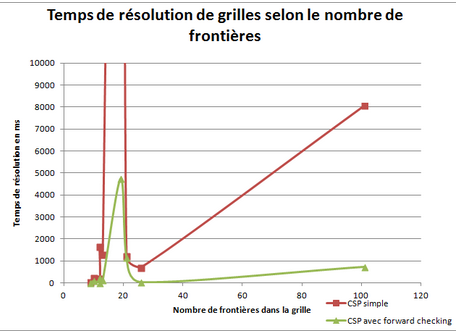
\includegraphics[scale=.5]{./vitesse.png}
\end{figure}

\section{Répartition des tâches}
\begin{enumerate}
        \item Martin: Interface et implémentation de l’algorithme de Backtracking, joueur artificiel aléatoire pour tester 
              l’interface, heuristique du nombre de drapeaux restants.
        \item Frédéric et Louis-Bertrand: Raisonnement probabiliste, heuristiques pour des cases aux mêmes probabilités.
        \item Nilovna et Geneviève: Documentation (lisez-moi, rapport), présentation, 
              revampage de l’interface, mises à l’essai, statistiques, nettoyage du code et remise.
\end{enumerate}

\section{Conclusion}
Les différentes études en intelligence artificielle visant à résoudre le jeu de démineur 
proposent une panoplie d’heuristiques. Il n’y a pas de doute que ce jeu, si simple en apparence, 
a une compléxité intéressante. Les membres de notre équipe se sont d’ailleurs amusés à continuer 
à améliorer les algorithmes utilisés jusqu’à la dernière minute. \\

Cette dernière remarque nous amène à parler des améliorations possibles que nous aurions souhaité apporter à notre programme:
\begin{enumerate}
        \item Modifier la façon dont la grille est générée afin de permettre à notre programme 
              de prendre une grille en entrée, ce qui nous aurait permis d’avoir des grilles fixes 
              lors des mises à l’essai, et donc de meilleures comparaisons entre les différents algorithmes;
        \item Le calcul des probabilités dans CrazyAI pourrait tenir compte des autres cases, 
              et donc la probabilité qu’une case soit minée ne serait pas fixe;
        \item L’heuristique des coins (commencer par les cases dans les coins puisqu’elles ont 
              moins de chance d’être adjacentes à une mine et tendent à révéler des régions complètes) 
              aurait pu être implémentée afin d’améliorer la performance de notre joueur artificiel;
        \item L’heuristique MCV (Most Constrained Value) aurait pu être implémentée dans le CSP : notre joueur 
              artificiel assumerait que chaque case non-découverte est minée et l’étiqueterait d’un drapeau. 
              Par la suite, il vérifierait si les contraintes sont satisfaites. Lorsqu’il trouverait qu’une 
              contrainte est insatisfaite (car il y aurait plusieurs drapeaux consécutifs qui totaliseraient 
              plus de mines possibles que les chiffres correspondants), il utiliserait l’heuristique MCV pour retirer des drapeaux.
\end{enumerate}

En ce qui concerne les apprentissages et les erreurs que nous avons commis lors de ce 
projet, mentionnons seulement le fait que nous avons d’abord opté pour la technique des 
réseaux bayésiens dans nos approches candidates, mais il s’est avéré qu’elle n’aurait pas
offert de meilleurs résultats que les autres algorithmes, pour beaucoup plus de travail. \\

En somme, notre algorithme allie satisfaction de contraintes et raisonnement probabiliste, imitant ainsi un joueur 
humain, ce qui représente un des principaux objectifs de l'intelligence artificielle.

\end{document}

